
\section{The Mersenne Twister: High-Dimensional Equidistribution}

Developed in 1997 by Makoto Matsumoto and Takuji Nishimura~\cite{matsumoto1998mersenne}, the Mersenne Twister (MT) is a widely used pseudorandom number generator in modern computing, serving as the default or standard option in software environments including Python's \texttt{random} module, R, MATLAB, and the C++ standard library.

By choosing parameters such that the effective state size $nw-r$ corresponds to a Mersenne exponent, the MT algorithm achieves a staggering periodicity and an extraordinarily high degree of multidimensional equidistribution.

\subsection{The Twisted Generalized Feedback Shift Register (TGFSR)}

The Mersenne Twister is based on Generalized Feedback Shift Register (GFSR). While a standard LFSR operates on single bits over $\mathbb{F}_2$, a GFSR operates on $w$-bit words, effectively running $w$ identical LFSRs in parallel.

The Mersenne Twister is a specific optimization of a \textit{Twisted} Generalized Feedback Shift Register (TGFSR). Let the word size be $w$ bits, and let the state array consist of $n$ words. The state at step $k$ is represented by a sequence of $w$-bit row vectors $\mathbf{x}_k \in \mathbb{F}_2^w$. 

\subsection{The Twist}
The TGFSR defines the state transition via a linear recurrence relation of order $n$. The generator computes the subsequent word $\mathbf{x}_{k+n}$ using the word from $n$ steps ago ($\mathbf{x}_k$) and a word from a mid-point $m$ steps ago ($\mathbf{x}_{k+m}$), augmented by a linear transformation matrix $A$:
\[
\mathbf{x}_{k+n} = \mathbf{x}_{k+m} \oplus \left( \mathbf{x}_k^u \mid \mathbf{x}_{k+1}^l \right) A
\]
Let us rigorously dissect the components of this linear transformation over $\mathbb{F}_2$:

\begin{description}
    \item[Concatenation ($\mid$):] The term $\left( \mathbf{x}_k^u \mid \mathbf{x}_{k+1}^l \right)$ represents a bitwise concatenation. We extract the upper $w-r$ bits from $\mathbf{x}_k$ (denoted $\mathbf{x}_k^u$) and the lower $r$ bits from the next state $\mathbf{x}_{k+1}$ (denoted $\mathbf{x}_{k+1}^l$). This creates a new, composite $w$-bit word. This incomplete word transition is one of the key innovations of the Mersenne Twister architecture, allowing the state space to precisely match a Mersenne prime rather than a power of 2.
    \item[The Matrix $A$:] The concatenated word is multiplied by a $w \times w$ matrix $A$ over $\mathbb{F}_2$. To ensure maximum computational efficiency in software, $A$ is chosen to be in Rational Normal Form (a companion matrix):
    \[
    A = \begin{pmatrix}
    0 & 1 & 0 & \cdots & 0 \\
    0 & 0 & 1 & \cdots & 0 \\
    \vdots & \vdots & \vdots & \ddots & \vdots \\
    0 & 0 & 0 & \cdots & 1 \\
    a_{w-1} & a_{w-2} & a_{w-3} & \cdots & a_0
    \end{pmatrix}
    \]
\end{description}

\begin{remark}
Because $A$ is in rational normal form, multiplying a vector $\mathbf{y} = (y_{w-1}, \dots, y_0)$ by $A$ can be executed via a single bit-shift and a conditional XOR. If the lowest bit $y_0 = 0$, the result is $\mathbf{y} \gg 1$. If $y_0 = 1$, the result is $(\mathbf{y} \gg 1) \oplus \mathbf{a}$, where $\mathbf{a} = (a_{w-1}, \dots, a_0)$. 
\end{remark}

\subsection{Tempering: Guaranteeing Equidistribution}

To avoid high degrees of linear correlation, failing rigorous tests for $k$-distribution, we add \textbf{tempering} to the process, which is an invertible linear transformation over $\mathbb{F}_2$. The tempering function $T: \mathbb{F}_2^w \to \mathbb{F}_2^w$ is designed to multiply the state vector by an invertible matrix $T$, which systematically scrambles the bits to achieve an optimal multidimensional distribution.

Given a raw state word $\mathbf{x}$, the tempered output $\mathbf{y}$ is generated through four successive shift-and-mask operations, utilizing shifting constants $(u, s, t, l)$ and bitmask vectors $\mathbf{a}, \mathbf{b}, \mathbf{c}, \mathbf{d}$:\begin{align*}
    \mathbf{y}_1 &= \mathbf{x} \oplus ((\mathbf{x} \gg u)
    \mathbin{\&} \mathbf{a}) \\
    \mathbf{y}_2 &= \mathbf{y}_1 \oplus ((\mathbf{y}_1 \ll s) \mathbin{\&} \mathbf{b}) \\
    \mathbf{y}_3 &= \mathbf{y}_2 \oplus ((\mathbf{y}_2 \ll t) \mathbin{\&} \mathbf{c}) \\
    \mathbf{y} &= \mathbf{y}_3 \oplus
    \left( (\mathbf{y}_3 \gg l) \mathbin{\&} \mathbf{d} \right)
\end{align*}
where $\mathbin{\&}$ denotes the bitwise AND operation.

\begin{theorem}
Because each step of the tempering process is an invertible linear transformation over $\mathbb{F}_2$, the composition of these transformations is likewise invertible. Hence, the entire tempering process defines a bijection on $\mathbb{F}_2^w$.
\end{theorem}

\subsection{Periodicity and Mersenne Primes}

The defining characteristic of the Mersenne Twister is its periodicity. The total number of bits in the internal state is $n \times w$. However, because $r$ bits are masked out during the concatenation step $\left( \mathbf{x}_k^u \mid \mathbf{x}_{k+1}^l \right)$, the actual operational state space consists of $nw - r$ bits. 

Therefore, the maximum possible period of the generator is $2^{nw - r} - 1$. 

\begin{definition}
A \textbf{Mersenne prime} is a prime number that can be written in the form $M_p = 2^p - 1$, where $p$ is a prime integer.
\end{definition}

By carefully choosing the parameters $n$, $w$, and $r$ such that $p = nw - r$ corresponds to the exponent of a Mersenne prime, Matsumoto and Nishimura simplified the mathematical analysis required to construct a primitive characteristic polynomial for the generator.

\subsection{Variants of the Mersenne Twister}

\subsubsection{The MT19937 Variant}
The most popular configuration of the Mersenne Twister is MT19937~\cite{matsumoto1998mersenne}. The parameters are chosen as follows:
\begin{itemize}
    \item Word size $w = 32$ bits.
    \item Degree of recurrence $n = 624$ words.
    \item Separation point $m = 397$.
    \item Lower bitmask size $r = 31$ bits.
\end{itemize}
This configuration results in a total operational state size of $624 \times 32 - 31 = 19937$ bits. The parameters of MT19937 were specifically selected so that the associated characteristic polynomial is primitive over $\mathbb{F}_2$, yielding the maximal possible period
\[
2^{19937} - 1.
\]
The fact that $19937$ is a Mersenne exponent plays an important role in the underlying construction and analysis.



\subsubsection{Other variants of the MT}
\begin{enumerate}
    \item \textbf{CryptMT:} CryptMT is a stream cipher and cryptographically secure pseudorandom number generator (CSPRNG). It was developed by Makoto Matsumoto and Takuji Nishimura alongside Mariko Hagita and Mutsuo Saito. Unlike the classical Mersenne Twister or its other structural derivatives, CryptMT is patented.
    
    \item \textbf{MTGP:} MTGP (Mersenne Twister for Graphics Processors) is a variant~\cite{saito2013mtgp} optimized for graphics processing units published by Mutsuo Saito and Makoto Matsumoto. The basic linear recurrence operations are extended from MT, and parameters are carefully chosen to allow a massive pool of parallel threads to compute the recursion concurrently while sharing their active state space to minimize memory load. The original paper claims improved multidimensional equidistribution over standard MT, displaying execution metrics on a 2008-era GPU (Nvidia GTX260 with 192 cores) of 4.7~ms to produce $5 \times 10^7$ random 32-bit integers.

    \item \textbf{SFMT:} SFMT (SIMD-oriented Fast Mersenne Twister) is a variant introduced in 2006 designed specifically to leverage speed advantages when executing on 128-bit SIMD architectures. It is roughly twice as fast as the classical Mersenne Twister. 

    \item \textbf{TinyMT:} TinyMT is a lightweight variant proposed by Saito and Matsumoto in 2011. It utilizes just 127 bits of internal state space, marking a significant footprint reduction compared to the 2.5~KiB state array required by the classic MT19937. However, its maximum period is bounded at:
    \[
    2^{127} - 1
    \]
    
\end{enumerate}



\subsection{C++ Implementation}

The core output operation of the Mersenne Twister is implemented in the \texttt{next()} method. When all words from the current state array have already been consumed, the generator first performs the twist step and rebuilds the internal state. Then it takes one raw 32-bit word from the state array and applies tempering.

\cppfile[
    caption={Output function of MT19937},
    label={lst:mt19937-next}
]{codes/mersenne_twister/mt19937_next.cpp}

The first part of the method checks whether the internal state array must be regenerated. This corresponds to applying the TGFSR recurrence described earlier. The variable \texttt{y} is then taken from the state array and transformed by four bitwise operations. These operations are the tempering step: right shifts, left shifts, XORs and bit masks are used to improve the distribution of output bits.

The important point is that the state transition and the output transformation are separated. The twist changes the internal state, while tempering changes only the returned value. Because tempering is invertible over $\mathbb{F}_2$, it improves the statistical quality of the visible output without changing the period of the underlying state cycle.

For comparison, two modified variants were also tested. The first one removes tempering and returns the raw state word directly.

\cppfile[
    caption={MT19937 output without tempering},
    label={lst:mt19937-no-tempering-next}
]{codes/mersenne_twister/mt19937_no_tempering_next.cpp}

The second modified variant removes the matrix constant from the twist operation. This keeps the output range large, but weakens the linear recurrence itself.

\cppfile[
    caption={MT-like output using a weakened twist step},
    label={lst:mt19937-bad-twist-next}
]{codes/mersenne_twister/mt19937_bad_twist_next.cpp}

\subsection{Experimental Comparison}

To illustrate the role of tempering and the twist matrix, three variants were compared. The first one is the standard MT19937 generator. The second one uses the same transition, but omits tempering. The third one uses a weakened twist step by removing the matrix constant $A$.

\begin{table}[htbp]
\centering
\small
\resizebox{\textwidth}{!}{%
\begin{tabular}{|l|r|r|r|}
\hline
Parameter & Standard MT19937 & No tempering & Bad twist matrix \\
\hline
Seed & $5489$ & $5489$ & $5489$ \\
Word size $w$ & $32$ & $32$ & $32$ \\
State size $n$ & $624$ & $624$ & $624$ \\
Middle word $m$ & $397$ & $397$ & $397$ \\
Lower mask bits $r$ & $31$ & $31$ & $31$ \\
Matrix constant $A$ & \texttt{0x9908B0DF} & \texttt{0x9908B0DF} & \texttt{0x00000000} \\
Tempering & yes & no & no \\
\hline
\end{tabular}%
}
\caption{Mersenne Twister variants used in the experiment}
\label{tab:mt-parameters}
\end{table}

For each generator, $100000$ generated values were used to compute basic statistics. The histogram was divided into $20$ buckets. The sequence plot and the successive-value plot were generated using $5000$ values.

\begin{table}[htbp]
\centering
\small
\resizebox{\textwidth}{!}{%
\begin{tabular}{|l|r|r|r|}
\hline
Statistic & Standard MT19937 & No tempering & Bad twist matrix \\
\hline
Min & $52150$ & $51092$ & $1008367$ \\
Max & $4294877384$ & $4294911316$ & $4294782864$ \\
Mean & $2143446744.27$ & $2148531592.69$ & $2199899818.70$ \\
Std. dev. & $1239920307.25$ & $1241945764.29$ & $1232324944.58$ \\
One-bit ratio & $0.499926$ & $0.500359$ & $0.500918$ \\
$\chi^2$ & $23.4012$ & $20.4104$ & $1512.2160$ \\
\hline
\end{tabular}%
}
\caption{Basic statistics computed from $100000$ outputs}
\label{tab:mt-statistics}
\end{table}

The standard MT19937 has a mean close to the middle of the 32-bit output range and a one-bit ratio very close to $0.5$. This indicates good balance between zeros and ones in the binary representation of generated values. The chi-square statistic for the histogram is also moderate, so the one-dimensional distribution looks close to uniform in this simple test.

The variant without tempering still looks acceptable in basic one-dimensional statistics. Its mean, standard deviation, bit ratio and histogram statistic are close to the standard version. This is expected, because removing tempering does not immediately destroy the period of the state transition. However, it exposes the raw linear structure of the state more directly, which is exactly what tempering is designed to hide.

The variant with the weakened twist matrix behaves much worse. Its chi-square statistic is much larger, even though the output range is still large. This shows that preserving a large numerical range is not enough. If the recurrence relation is weakened, the generator may produce visibly non-uniform bucket frequencies and stronger structural artifacts.

\subsection{Plots and Interpretation}

\begin{figure}[htbp]
\centering
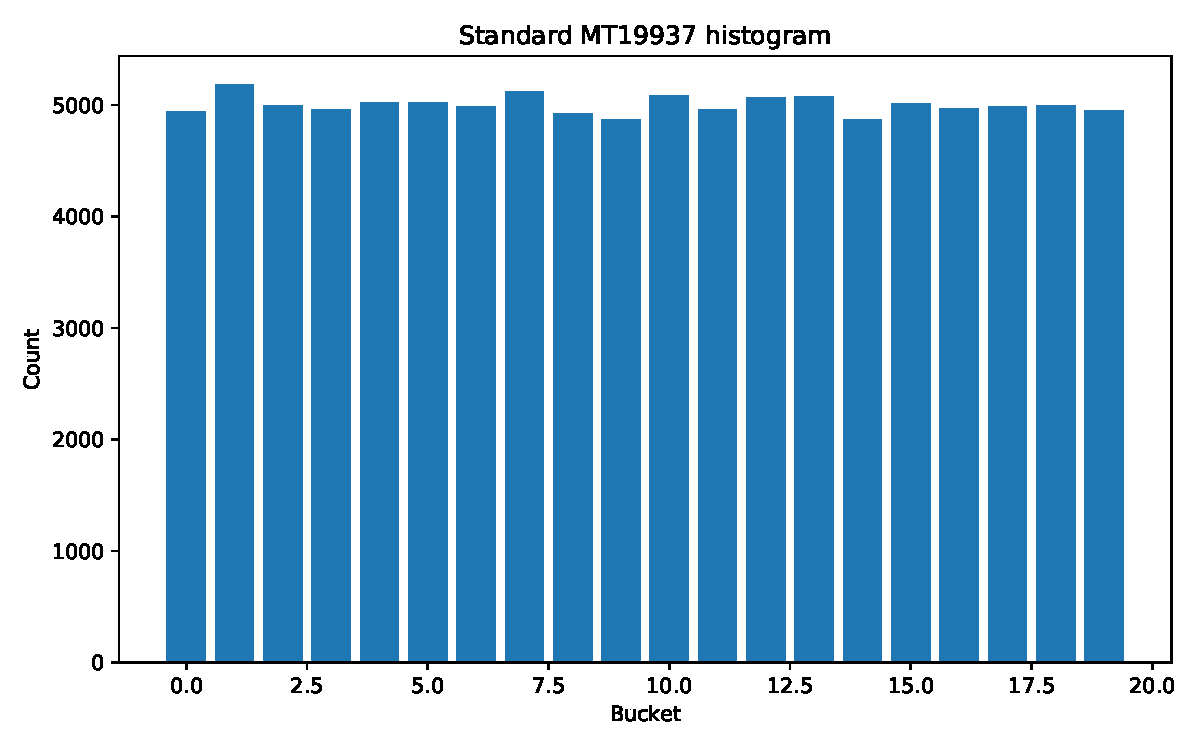
\includegraphics[width=0.48\textwidth]{figures/mersenne_twister/good/mt19937_good_histogram.pdf}
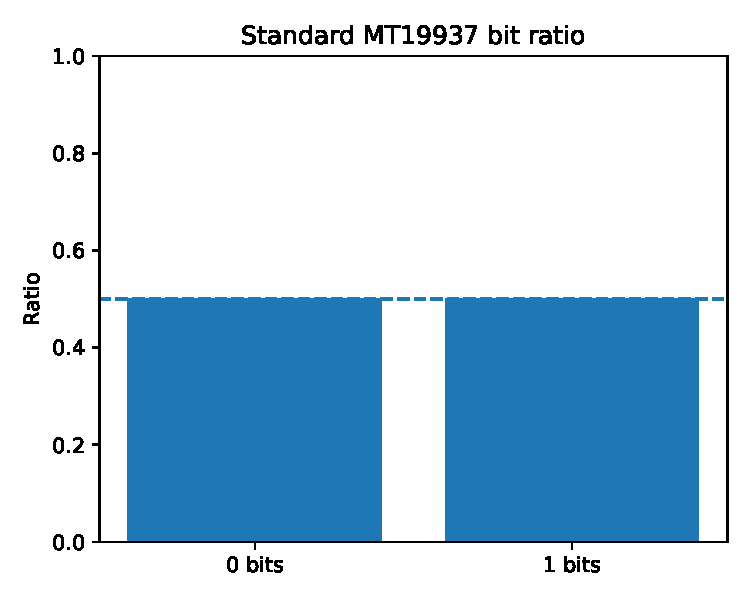
\includegraphics[width=0.48\textwidth]{figures/mersenne_twister/good/mt19937_good_bit_ratio.pdf}
\caption{Histogram and bit ratio for the standard MT19937}
\label{fig:mt-good-hist-bits}
\end{figure}

Figure \ref{fig:mt-good-hist-bits} shows that the standard MT19937 distributes values evenly across the histogram buckets. The bit-ratio plot is almost exactly centered at $0.5$, which confirms that zeros and ones occur with nearly equal frequency.

\begin{figure}[htbp]
\centering
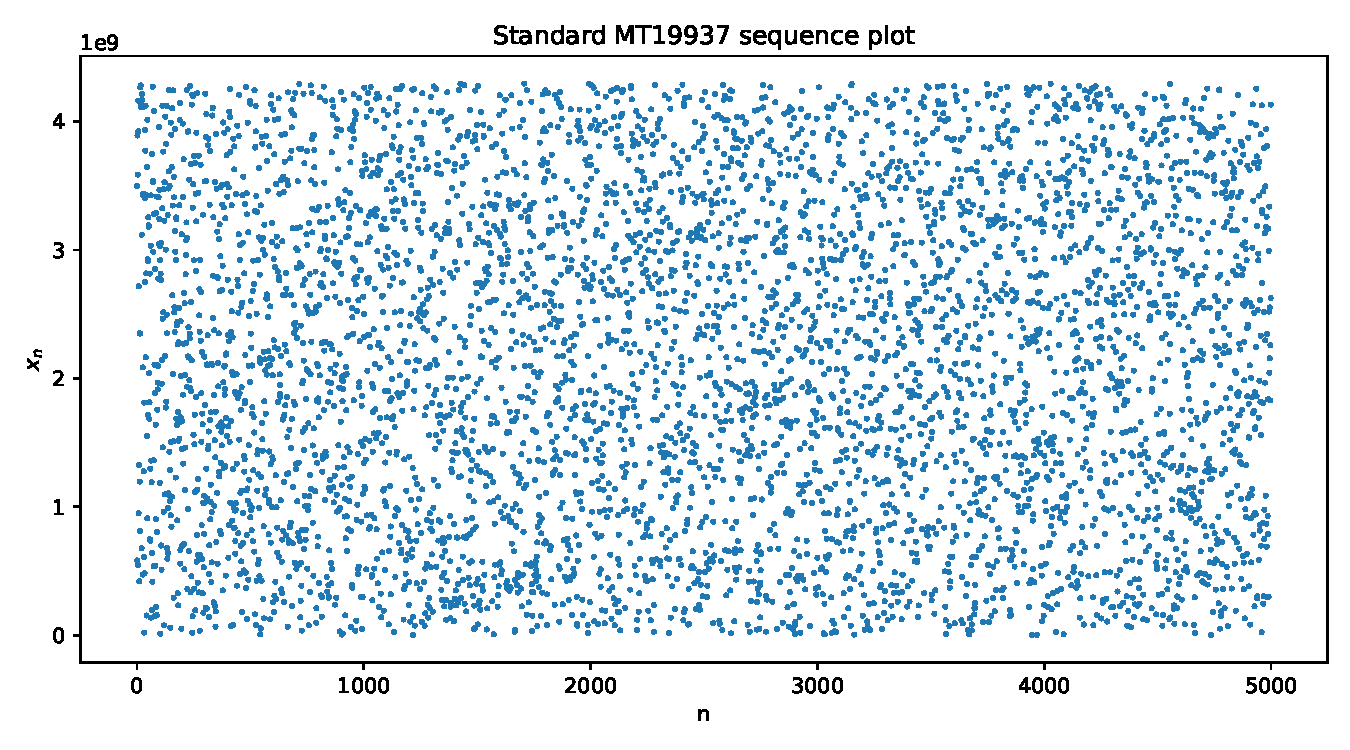
\includegraphics[width=0.48\textwidth]{figures/mersenne_twister/good/mt19937_good_sequence.pdf}
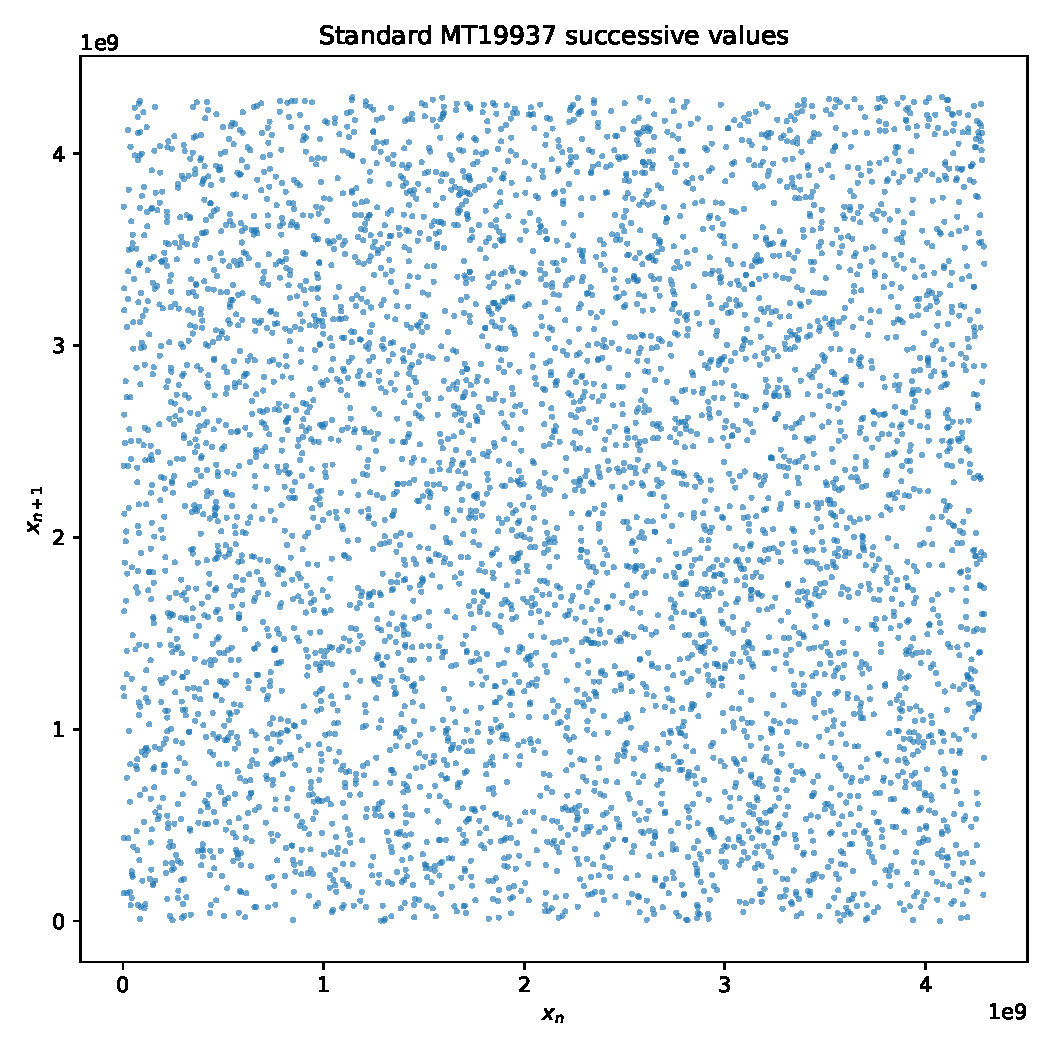
\includegraphics[width=0.48\textwidth]{figures/mersenne_twister/good/mt19937_good_successive_values.pdf}
\caption{Sequence plot and successive-value plot for the standard MT19937}
\label{fig:mt-good-sequence-successive}
\end{figure}

Figure \ref{fig:mt-good-sequence-successive} shows that the generated values cover the full 32-bit range. The successive-value plot does not collapse into a small set of visible lines, which is consistent with the high-dimensional equidistribution properties of MT19937.

\begin{figure}[htbp]
\centering
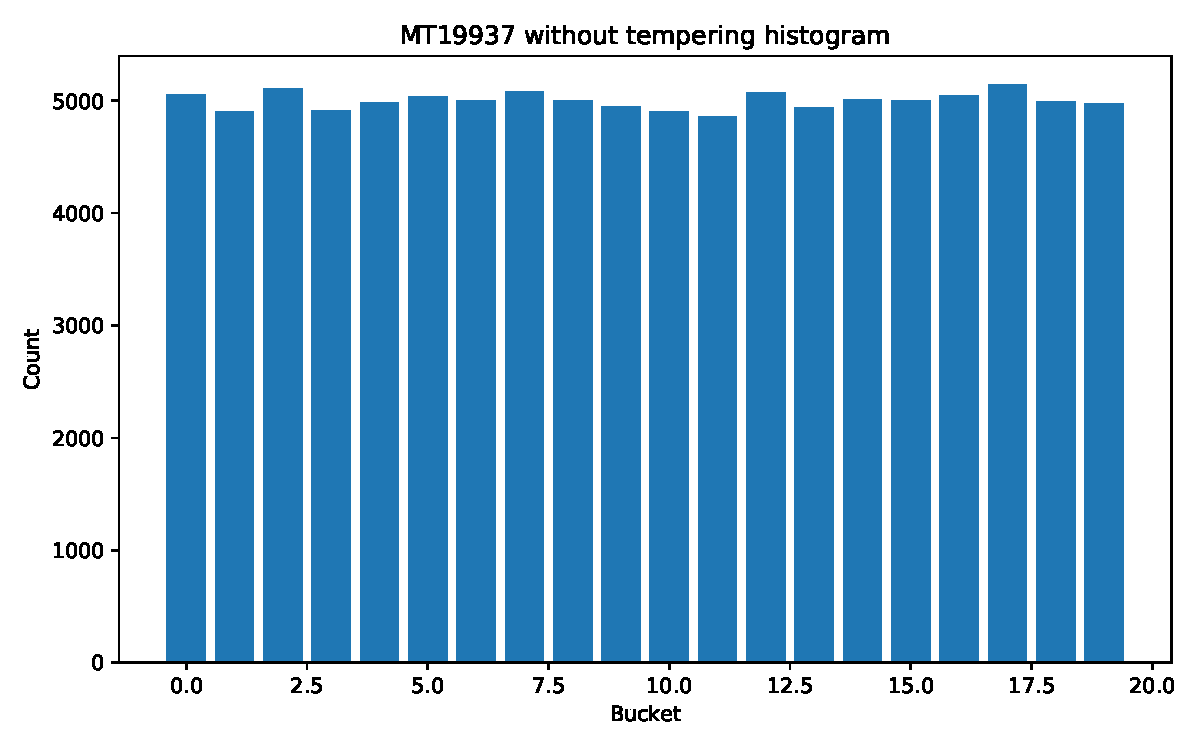
\includegraphics[width=0.48\textwidth]{figures/mersenne_twister/single_bad_parameter/mt19937_no_tempering_histogram.pdf}
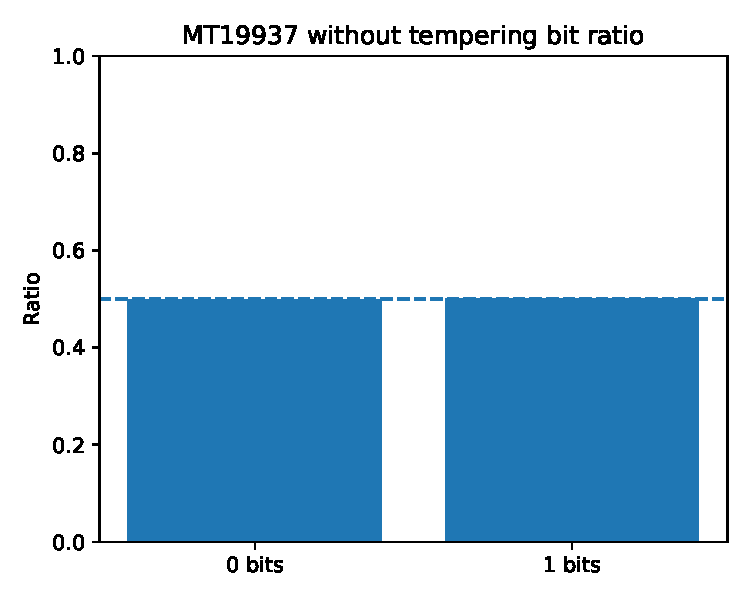
\includegraphics[width=0.48\textwidth]{figures/mersenne_twister/single_bad_parameter/mt19937_no_tempering_bit_ratio.pdf}
\caption{Histogram and bit ratio for MT19937 without tempering}
\label{fig:mt-no-tempering-hist-bits}
\end{figure}

Figure \ref{fig:mt-no-tempering-hist-bits} shows that removing tempering does not necessarily create an obvious failure in a simple histogram. This is a useful example of a generator that may look acceptable in basic tests, while still being theoretically weaker because the raw linear state is exposed.

\begin{figure}[htbp]
\centering
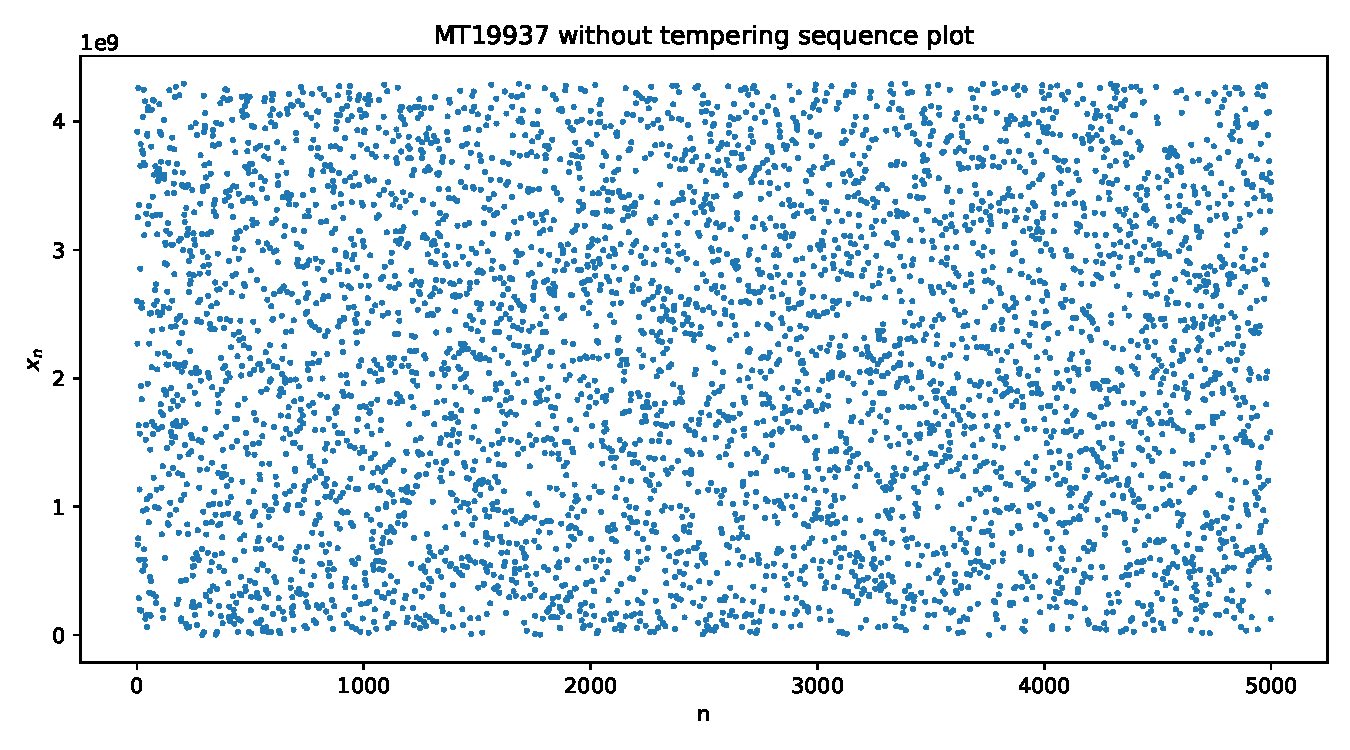
\includegraphics[width=0.48\textwidth]{figures/mersenne_twister/single_bad_parameter/mt19937_no_tempering_sequence.pdf}
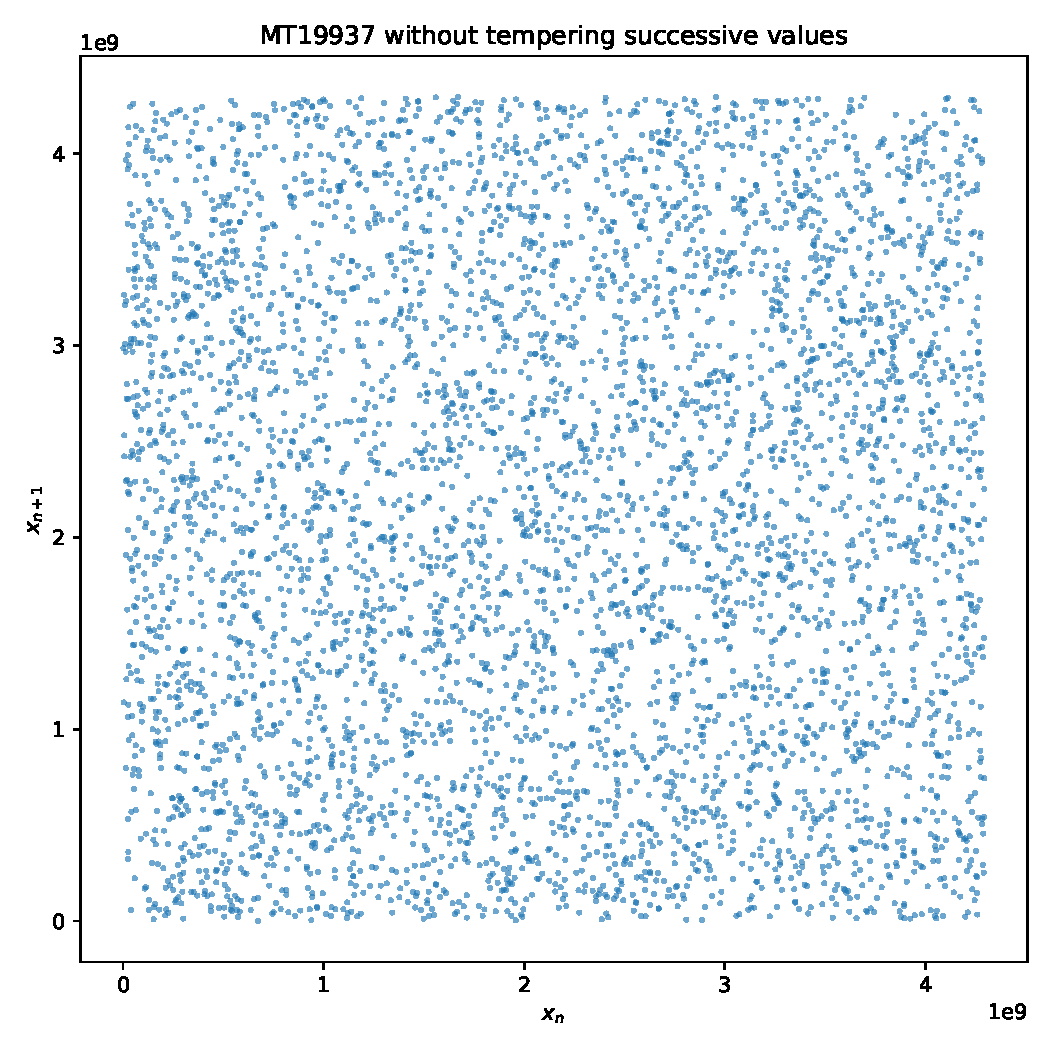
\includegraphics[width=0.48\textwidth]{figures/mersenne_twister/single_bad_parameter/mt19937_no_tempering_successive_values.pdf}
\caption{Sequence plot and successive-value plot for MT19937 without tempering}
\label{fig:mt-no-tempering-sequence-successive}
\end{figure}

Figure \ref{fig:mt-no-tempering-sequence-successive} again shows that short visual tests are limited. The values still cover a broad range, but without tempering the output is a more direct observation of the internal linear recurrence.

\begin{figure}[htbp]
\centering
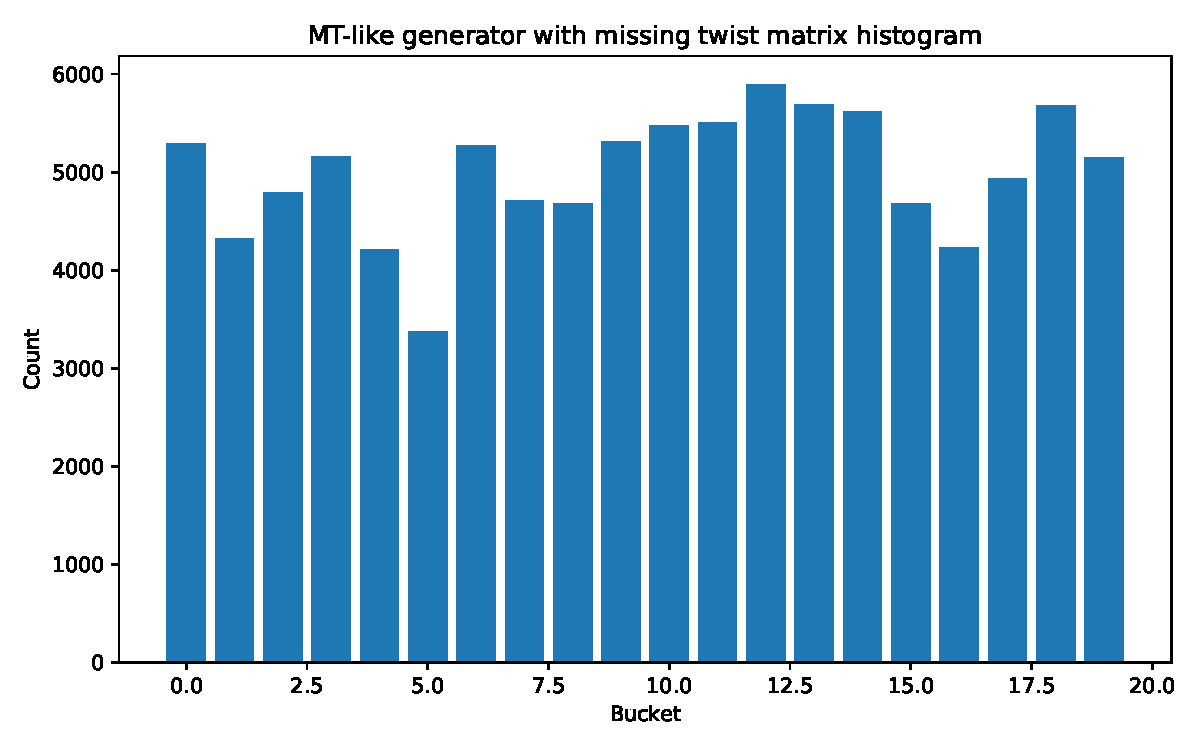
\includegraphics[width=0.48\textwidth]{figures/mersenne_twister/bad_large_range/mt19937_bad_twist_histogram.pdf}
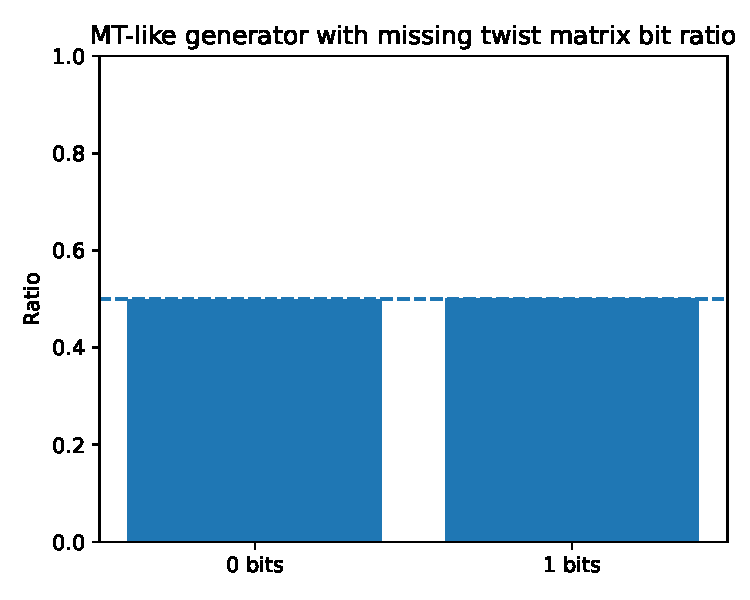
\includegraphics[width=0.48\textwidth]{figures/mersenne_twister/bad_large_range/mt19937_bad_twist_bit_ratio.pdf}
\caption{Histogram and bit ratio for the MT-like generator with weakened twist}
\label{fig:mt-bad-twist-hist-bits}
\end{figure}

Figure \ref{fig:mt-bad-twist-hist-bits} shows the clearest failure. The bit ratio is still close to $0.5$, but the histogram is visibly less uniform. This demonstrates that bit balance alone is not sufficient to judge the quality of a pseudorandom generator.

\begin{figure}[htbp]
\centering
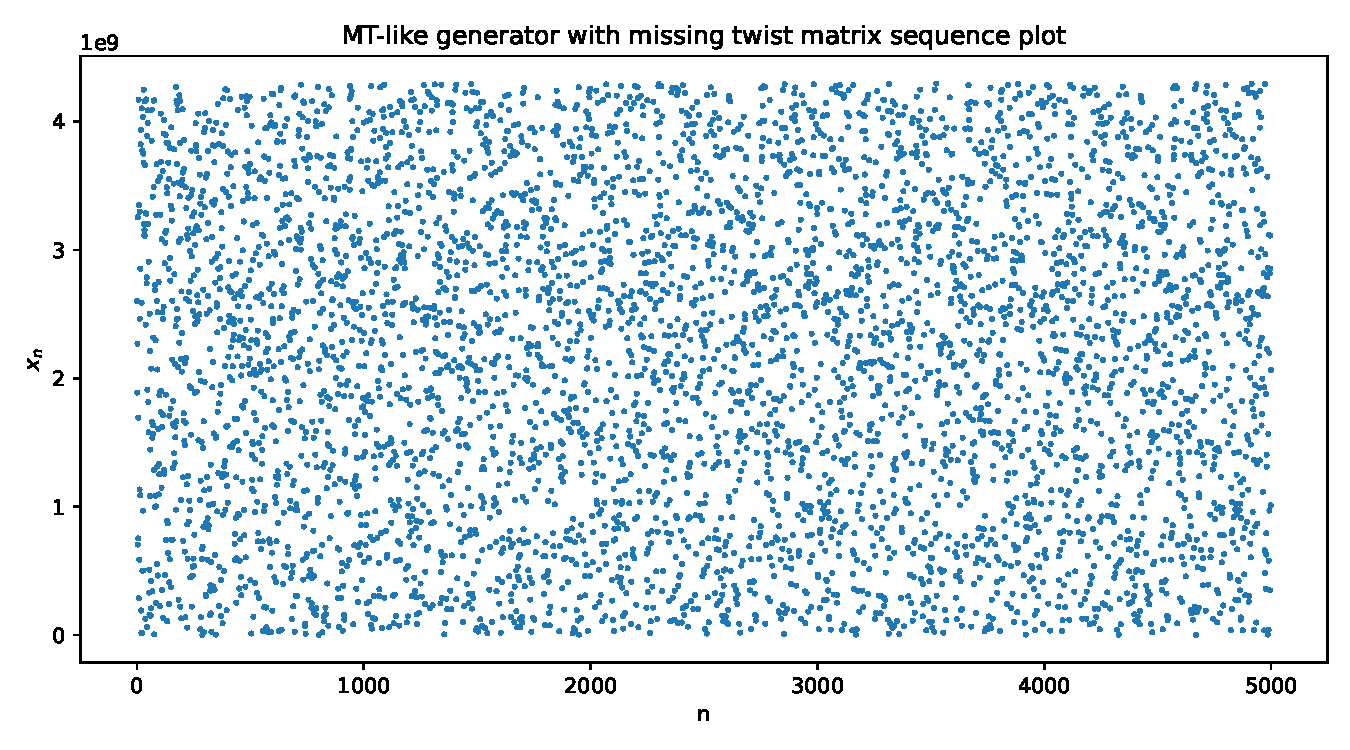
\includegraphics[width=0.48\textwidth]{figures/mersenne_twister/bad_large_range/mt19937_bad_twist_sequence.pdf}
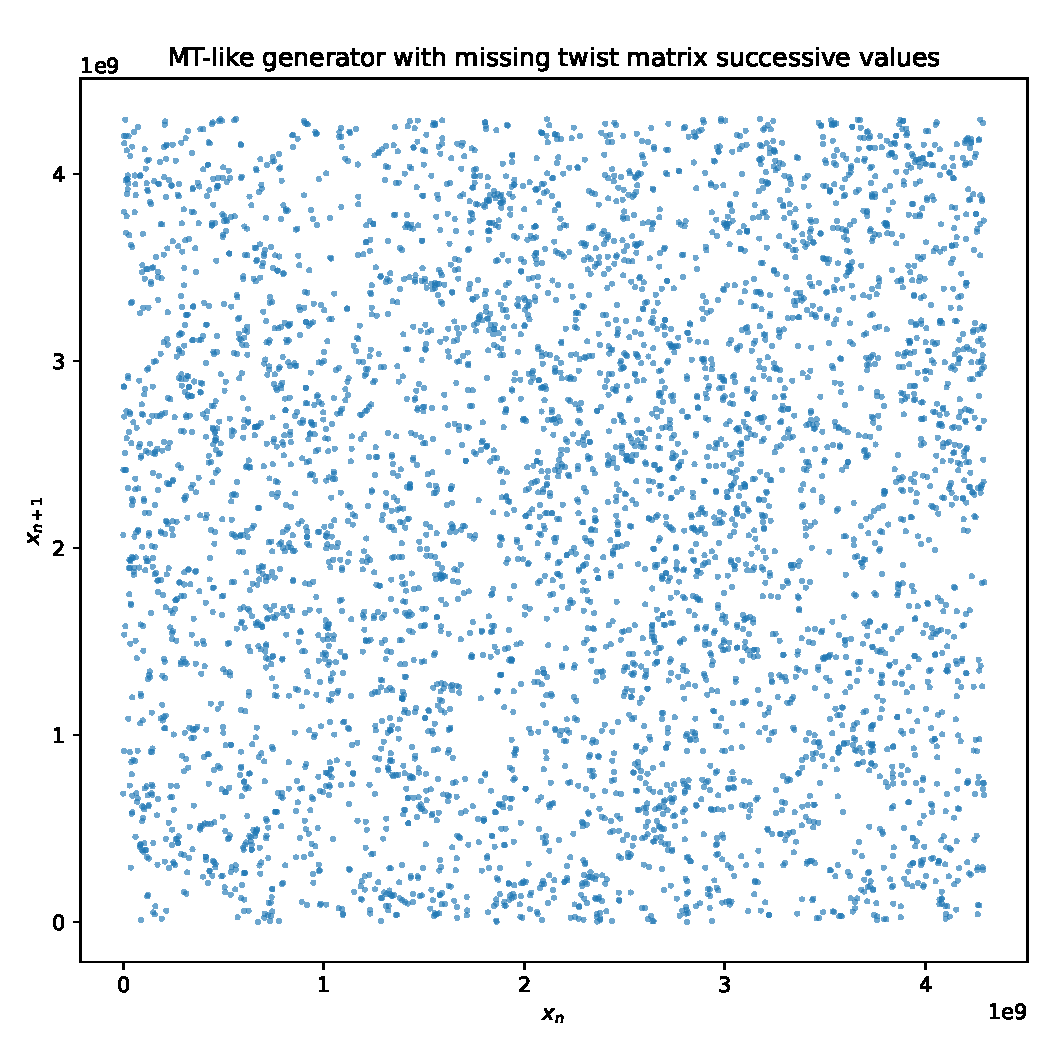
\includegraphics[width=0.48\textwidth]{figures/mersenne_twister/bad_large_range/mt19937_bad_twist_successive_values.pdf}
\caption{Sequence plot and successive-value plot for the MT-like generator with weakened twist}
\label{fig:mt-bad-twist-sequence-successive}
\end{figure}

Figure \ref{fig:mt-bad-twist-sequence-successive} illustrates that the weakened recurrence still produces values from a large range, but the distributional behavior is worse. The comparison confirms that both parts of the Mersenne Twister construction are important: the twist step determines the quality of the state transition, while tempering improves the visible output distribution.

Overall, the experiment shows that MT19937 works well not because of a single operation, but because its parameters, recurrence relation and tempering transformation are carefully chosen together. Removing one part may not always break simple statistics immediately, but it weakens the structural properties that make the generator reliable in larger simulations.
